\documentclass[12pt]{article}

\usepackage{sbc-template}

\usepackage{graphicx,url}

\usepackage[brazil]{babel}
\usepackage[utf8]{inputenc}
\usepackage[T1]{fontenc}
     
\sloppy

\title{Projeto Integrador IV: Extração e Visualização de Dados\\ CrawlerJobs}

\author{Humberto Vieira de Castro\inst{1}, Mario Roberto de Castro\inst{1}, Paulo Henrique Leite\inst{1}}

\address{Ciências da Computação -- Centro Universitário Senac São Paulo
  (SENAC-SP)\\
  Av. Engenheiro Eusébio Stevaux, 823, São Paulo -- SP
\email{\{humbertovieira.castro, marico.castro, leite.paulohf\}@gmail.com}
}

\begin{document} 

\maketitle

\begin{abstract}
(Pedir pra laurana traduzir)
Este artigo descreve o trabalho relativo ao desenvolvimento de um web Crawler com o objetivo de extrair dados nos principais sites de empregos no Brasil. Além disto, é apresentado a solução proposta pela equipe  em relação a visualização dos dados extraídos, uma parte muito importante do projeto desenvolvido. O artigo detalha toda a elaboração do projeto, trazendo seus aspectos técnicos, as dificuldades encontradas na implementação, os recursos pedagógicos utilizados, algoritmos implementados e o resultado final obtido.
\end{abstract}
     
\begin{resumo} 
Este artigo descreve o trabalho relativo ao desenvolvimento de um web Crawler com o objetivo de extrair dados nos principais sites de empregos no Brasil. Além disto, é apresentado a solução proposta pela equipe  em relação a visualização dos dados extraídos, uma parte muito importante do projeto desenvolvido. O artigo detalha toda a elaboração do projeto, trazendo seus aspectos técnicos, as dificuldades encontradas na implementação, os recursos pedagógicos utilizados, algoritmos implementados e o resultado final obtido.
\end{resumo}

\section{Introdução}

O objetivo deste trabalho é o desenvolvimento de um web crawler que seja capaz de extrair dados dos principais sites de empregos. Além disto, ele também é utilizado para manter a base de dados sempre atualizada.

Para armazenar todos os dados extraídos pelo crawler, foi usado um banco de dados relacional, através deste, é possível gerenciar todo o conteúdo obtido e garantir a integridade dos dados.

Após a mineração e normalização das informações obtidas, foi desenvolvido um site para a visualização destes dados. A visualização foi criada a partir do processing.js, este faz uma ponte entre processing e javaScript, permitindo a criação gráfica de dados em 2d e 3d.

Afim de trazer a melhor experiência para os usuários, foi criado algumas personas para executar testes de usabilidade.  Através destas, é possível perceber padrões de dificuldade entre usuários durante a navegação. Com os padrões estabelecidos, a criação de uma plataforma simples e usual para todos se torna mais fácil.

\section{O projeto}

Anualmente, milhões de profissionais utilizam sites de empregos para conseguir entrar no mercado de trabalho e através destes é possível ter acesso a mais de 2 milhões de vagas para se candidatar, estas são diariamente publicadas por mais de 100 mil empresas registradas no mercado brasileiro, segundo a Catho.

Com o objetivo de analisar o mercado brasileiro, foi desenvolvido um sistema que busca vagas de empregos armazenadas nos principais sites de contratação (Catho, infoJobs, Manager e Empregos), através deste é possível verificar informações de salário médio por cargo, região e cidade, as profissões mais procuradas pelas empresas no momento atual e até mesmo a escolaridade e requisitos mais procurados por elas.

\subsection{Etapas do projeto} \label{sec:firstpage}

A primeira parte do projeto remetesse ao desenvolvimento de um web Crawler capaz de minerar dados nas principais plataformas de empregos. As plataformas escolhidas pela equipe foram: Catho, infoJobs, Manager e Empregos.

A segunda etapa consiste no tratamento das informações extraídas,  buscando padrões e fazendo a devida separação dos dados por categorias. Após este tratamento, o conteúdo será inserido em um banco de dados responsável em armazenar e manter as informações sempre atualizadas.

A terceira etapa consiste em um trabalho de visualização de dados, onde uma plataforma de visualização gráfica deverá ser desenvolvida para permitir que o usuário acesse as informações derivadas do banco de dados.

\section{Desenvolvimento}\label{sec:figs}

(Em desenvolvimento)

\subsection{Dificuldades e soluções}

O projeto é constituído por dois grandes desafios, a extração de dados feita através de um crawler e a visualização deste conteúdo. 

(Em desenvolvimento)

Outro problema encontrado pela equipe durante o desenvolvimento do projeto foi em relação ao robots.txt, como o próprio nome já diz, robots.txt é um arquivo de texto que funciona como filtro para os robôs dos sites de busca, ou seja, para o seu crawler. Ele tem como função controlar as permissões de acesso as páginas dos sites, informando quais dados podem ou não serem indexados.

É importante lembrar que o robots.txt não previne que o crawler acesse os diretórios e arquivos dos sites, ele funciona mais como uma espécie de placa na porta de entrada, dizendo o que pode ou não ser acessado, ou seja, é necessário que a pessoas tenha bom senso moral e ético para respeitar a placa.

\subsubsection{Extração de dados usando API}

Para projetos que estão começando, onde tempo é um problema, a API pode ser uma grande aliada, pois além de ser algo simples de utilizar, contribui para o crescimento do seu projeto, tornando-o mais completo.

Ao desenvolver um crawler, deve ser levado em consideração a forma que os dados estão sendo obtidos, em geral, é possível obter as informações desejadas de várias formas diferentes, como por exemplo, extrair os dados diretamente de um HTML, entretanto, para assegurar a durabilidade do crawler desenvolvido, é preferível a escolha de uma plataforma que possua uma API própria para esse tipo de serviço, caso contrário, se ocorrer alterações no HTML, o sistema de mineração pode ser comprometido e parar de funcionar, neste caso, deve ser feito alguns tratamentos no processo de extração para dificultar esta depreciação.

(Em desenvolvimento)

\subsubsection{Extração de dados usando HTML}

(Em desenvolvimento)

\subsubsection{Criação de um web crawler}

(Em desenvolvimento)

\subsubsection{Escolhendo a visualização de dados}

(Em desenvolvimento)

\subsection{Aprendizado de novas tecnologias}

(Em desenvolvimento)

\subsubsection{Node.js}

(Em desenvolvimento)

\subsubsection{Plataforma Azure}

(Em desenvolvimento)

\subsubsection{Linguagem SQL}

(Em desenvolvimento)

\subsubsection{Processing.js}

(Figure~\ref{fig:exampleFig1} Em desenvolvimento).

\begin{figure}[ht]
\centering
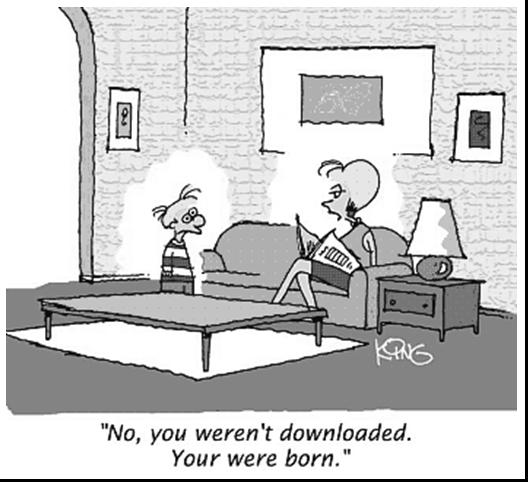
\includegraphics[width=.5\textwidth]{fig1.jpg}
\caption{Figura exemplo - Em desenvolvimento.}
\label{fig:exampleFig1}
\end{figure}

\section{Resultados e discussões}

(Em desenvolvimento)

\section{References}

Bibliographic references must be unambiguous and uniform.  We recommend giving
the author names references in brackets, e.g. \cite{knuth:84},
\cite{boulic:91}, and \cite{smith:99}.

The references must be listed using 12 point font size, with 6 points of space
before each reference. The first line of each reference should not be
indented, while the subsequent should be indented by 0.5 cm.

\bibliographystyle{sbc}
\bibliography{sbc-template}

\end{document}